\section{Design}

\subsection{System Architecture}

As discussed during the planning stages, Choona will be built using the microservices architecture. Figure \ref{fig:architecture} shows the proposed system design for Choona, split into four layers.

\begin{figure}[h!]
  \centering
  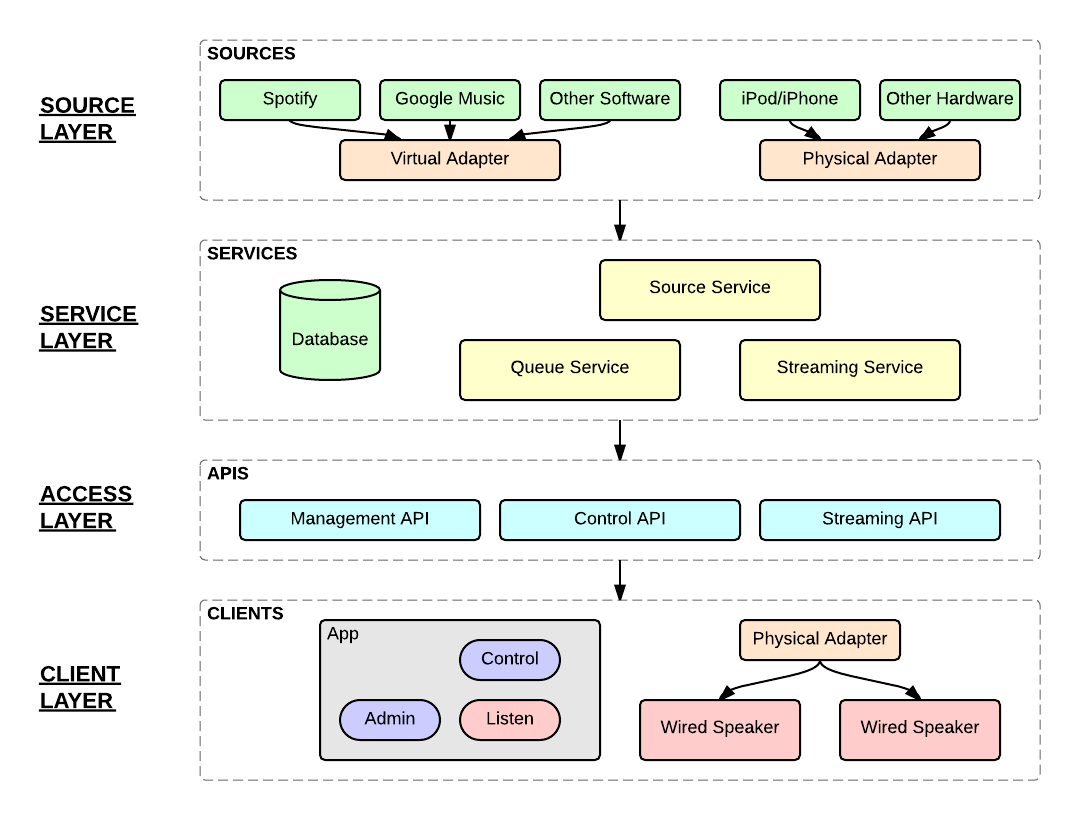
\includegraphics[width=1\textwidth]{./img/sys-architecture.png}
  \caption{Proposed Choona system architecture}
  \label{fig:architecture}
\end{figure}

\begin{itemize}
  \item \textbf{Source Layer}\\
    Sources, such as Spotify and Google Music, all have their own unique APIs. For them to be consumed by Choona they need to present a common interface otherwise other services will need to know how to interact directly with each individual API. Therefore each source will be exposed through either a virtual or physical adapter. Each adapter understands the same set of commands and outputs data in the same format. This means that other services in Choona only need to implement the standard adapter interface in order to communicate with any type of audio source. For the first version of Choona the sources will only need to understand a basic set of instructions:
    \begin{itemize}
      \item \texttt{search [searchString]} - search the source's track database using the supplied search string
      \item \texttt{get [trackId]} - retrieve track information from the source's database for the specified track ID
      \item \texttt{play [trackId]} - stream the audio for the specified track ID
    \end{itemize}

  \item \textbf{Service Layer}\\
    The service layer contains the majority of the \textit{business logic} of the Choona server-side infrastructure. There will be three main services at this layer. The queue service is responsible for maintaining the running playlist of tracks for a particular Choona location. The source service acts as an interface to all the different types of audio sources (instructions documented above). The streaming service takes tracks from the queue service, retrieves the audio via source service and sequences it into a single stream that the APIs can then send to clients. This layer has a more extensive set of instructions:
    \begin{itemize}
      \item \texttt{queue join [locationId] [clientId]} - make a client join a particular location
      \item \texttt{queue add [locationId] [trackId]} - add a song to the queue of a particular location
      \item \texttt{queue upvote [locationId] [trackId]} - upvote a song at a particular location
      \item \texttt{queue downvote [locationId] [trackId]} - downvote a song at a particular location
      \item \texttt{stream add [locationId] [trackId]} - instruct the streaming service to play a particular track next at a certain location
      \item \texttt{stream play [locationId]} - broadcast the stream to all listening clients of a location
    \end{itemize}

  \item \textbf{Access Layer}\\
    The access layer contains APIs that clients can use to interact with the Choona infrastructure. These APIs act as proxies, taking requests from clients and passing them through to the right services in the service layer. The only special instruction the access layer makes available is user authentication verification.

  \item \textbf{Client Layer}\\
    The client layer contains all the consumers of Choona, such as the mobile app and speaker adapter. Clients use the access layer to authenticate and interact with the rest of the Choona infrastructure; they do not need to know about all the individual services, instead they only need to understand the access APIs.
\end{itemize}

\subsection{UI Design}

\subsubsection*{Global Styling}

\noindent\underline{Colour schemes}\newline
There are a number of different colour schemes that can be used for the app, these must be discussed to make sure the most appropriate colour scheme is chosen.  This should line up with our literature and satisfy our target market needs.

To quickly review, as discussed in the literature review a dark user interface is more appropriate for choona because it:
\begin{itemize}
\item Is quite popular, adds a certain elegance to the app.
\item Is more convenient because the app will be used in illuminated and unilluminated environments (such as nightclubs and concerts). White background here may be too bright to look at and may strain the eyes.
\item Conserves battery life on the users phone.
\end{itemize}

\noindent However on the other hand there are some advantages to a light user interface:
\begin{itemize}
\item Better readability; even though this is not strictly a text-heavy application, the text involved will be easier to read on a lighter background with a contrasting text colour
\end{itemize}

\noindent Furthermore, we also found we should:
\begin{itemize}
\item Not use a scheme with too high a contrast; white text on a black background and vice versa should be avoided.
\item Keep the colour scheme minimal; busy colour scheme will dim the background and sharpen the contrast.
\end{itemize}

Taking all this into account we can start playing with a couple of different colour schemes that are friendly with our research. Each colour scheme will consist of 3 colours; background colour, text colour and highlight colour. 

The first colour scheme is to try to give the app a light user interface. The colours trialled here are a light grey (\#DDDDDD) with black (\#000) for text and light blue (\#009CFF) for highlighting elements. This does bring optimal readability to the table for choona however it can be argued that its not a text-heavy application so maybe readability is a high priority.\\

\begin{figure}[h!]
    \centering
        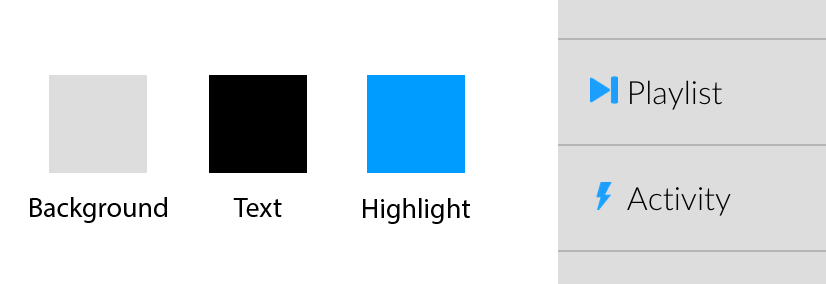
\includegraphics[width=0.8\textwidth]{./img/greybluecolours.png}
        \caption{Light grey, black and light blue}
        \label{fig:bluegrey}
\end{figure}

The second colour scheme sways more towards a dark UI. The background would be a dark grey (\#191919)  with white (\#FFF) for text and orange (\#FE6718) to highlight elements. This would fit into the dark UI scheme as talked about earlier but also because the orange signifies a community feeling. This is perfect for the concept of choona as one of its aims is to bring people together with the power of music. \\

\begin{figure}[h!]
\centering
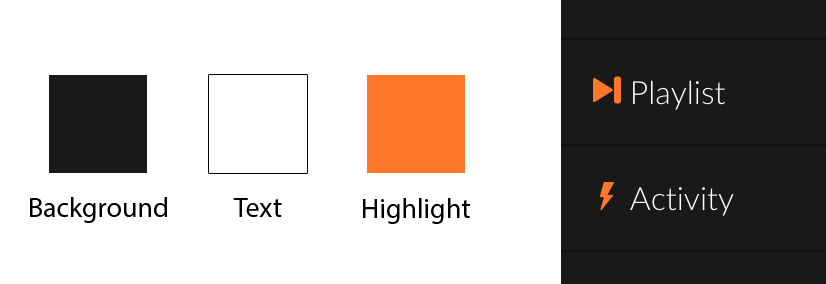
\includegraphics[width=0.8\textwidth]{./img/greyorangecolours.png}
\caption{Dark grey, white and orange}
\label{fig:orangegrey}
\end{figure}

The orange fits in better as a highlighting colour as it is quite a bright colour. Bright colours should not be over used because then they would become a distraction and cause problems in terms of readability.  \\

\noindent\underline{Choona Logo}\newline
The logo for any business is used as a method to not only identify the business but also set it apart from others. The name `Choona' is a play on the word `Choon' which is slang to describe a song or a `Tune', it also sounds like `Tuna' thus we thought the logo should be a fish. As the look and feel of the app is quite minimal, the logo should be quite minimal too. However we did not want our logo to just be a fish, looking at how a usual WiFi signal logo is designed, we thought that would be the perfect tail for the fish as WiFi represents a network of people much like Choona does. After a very simple fish being drawn, a WiFi tail was added and the image was rotated to look up, then the image was coloured to better go with the global colour scheme picked for the app. The tail will be animated in the app. This is shown in figure \ref{fig:logo}.

\begin{figure}[h!]
\centering
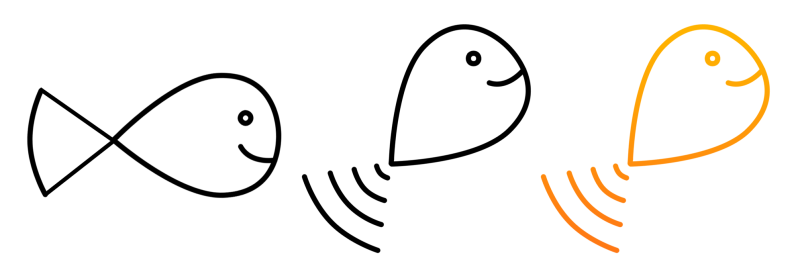
\includegraphics[width=0.5\textwidth]{./img/logothinking.png}
\caption{Thoughts behind the Choona logo}
\label{fig:logo}
\end{figure}


\noindent\underline{Font}\newline
There are a number of different fonts that can be considered for the application. There was a section already covered in the literature review regarding fonts. The font to be used should be clean and work well with the background and the theme of the application. Text needs to be sized appropriately so its not too big to take screen real estate but big enough for the users to read.

The first consideration is a font called BONVENOCF shown in figure \ref{fig:Bonvenocf}. This font consists of a clean font face ideal for minimal design. It's not the conventional type of font, there are some characters which possess a more rounded feel than the usual fonts. It's uniqueness will be fitting for the app; a unique looking font for a unique app. 

\begin{figure}[h!]
\centering
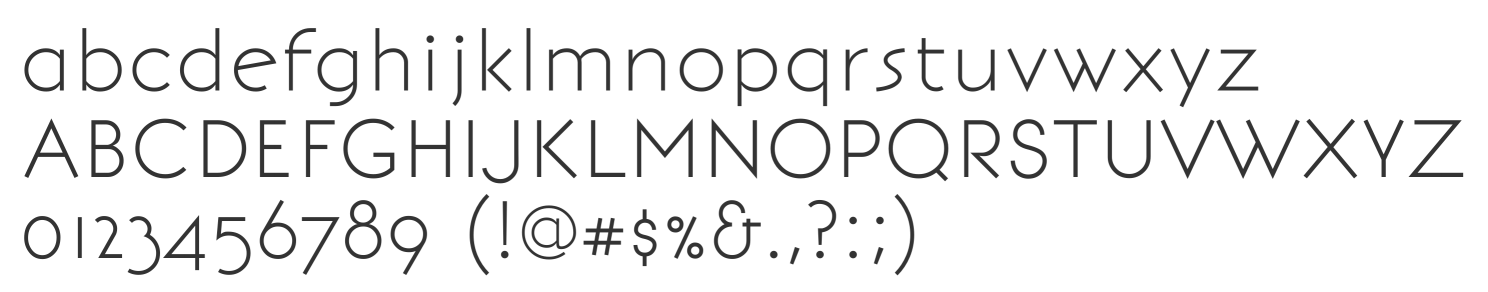
\includegraphics[width=0.55\textwidth]{./img/bonvenocf.png}
\caption{Bonvenocf font\footcite{bonvenocf}}
\label{fig:Bonvenocf}
\end{figure}

Next, Google's Lato font is another option shown in figure \ref{fig:lato}. This font is used globally; with Google handling over 3 billion serves every week through their font API\footcite{googlelato}. This shows that users are very familiar to this font and just by looking at the statistics its wide usage indicates the easy readability of the font.

\begin{figure}[h!]
\centering
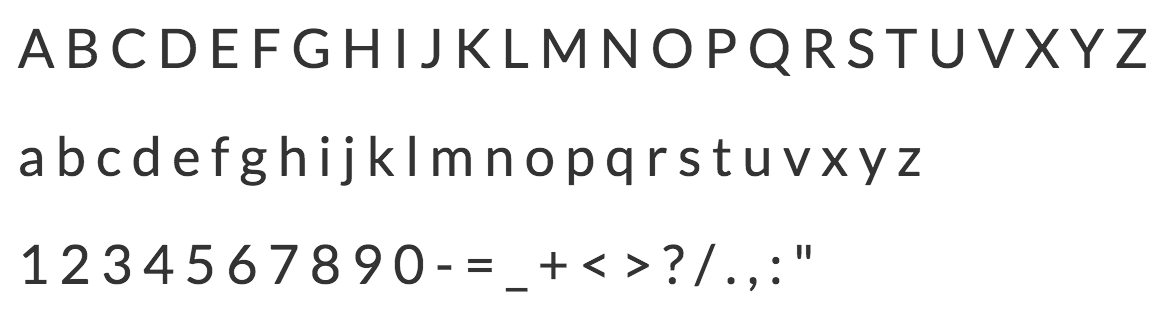
\includegraphics[width=0.65\textwidth]{./img/lato.png}
\caption{Lato font\footcite{googlelato}}
\label{fig:lato}
\end{figure}

Out of the two fonts, we believe Lato is the better fit for the application, with its clean minimal approach fitting in perfectly with the choona ecosystem.  The statistics speak for themselves; there is a clear reason this font is widely used.\\

\subsubsection*{UI Mock-ups}

The different pages of the app will be looked at closely, discussing different elements of the page in question and the reasoning behind any design decisions taken. This section will also make clear the general overall aesthetics that choona has employed to make the user's life much easier while maintaining a sleek clean look.\\

\clearpage

\noindent\underline{Welcome pages}\newline

The welcome pages will be shown to the user when they first install the app so they can quickly familiarise themselves with what it is about. Here information should be very clear and very simple as this is the first thing the user will see; they do not want to be overloaded with information. \\

\noindent
\begin{figure}[h!]
\centering
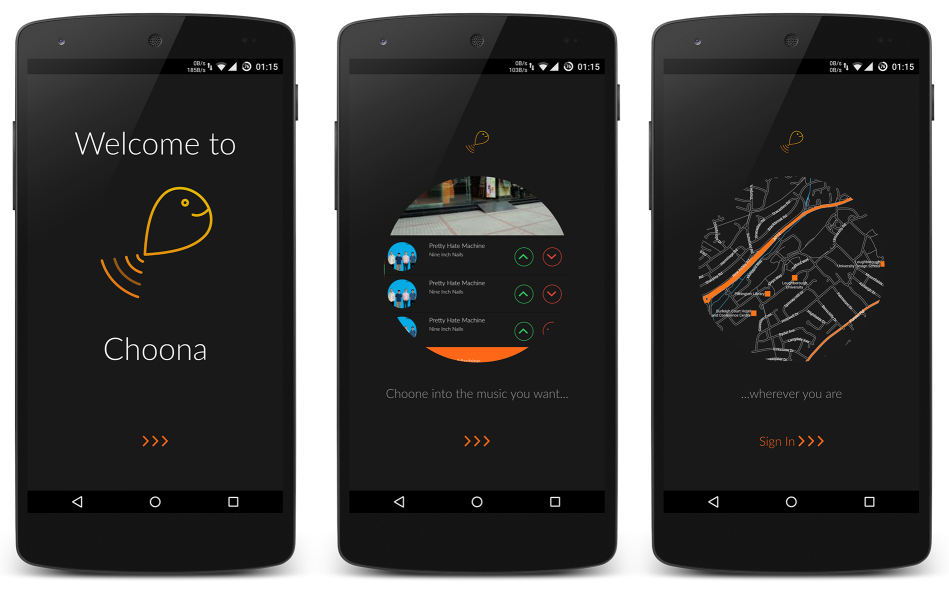
\includegraphics[width=0.95\textwidth]{./img/welcomeframed.png}
\caption{Welcome screens}
\label{fig:welcomescreens}
\end{figure}

Here the idea is to use multiple `slides' that the user can swipe through to reach the welcome screens. As shown in figure \ref{fig:welcomescreens} the users are first greeted with the Choona logo and a welcome message before moving onto two screens that describe what Choona does in one phrase; `Choon into the music you want....wherever you are'. These screens are split as this gives the chance to display the playlist page and a geolocation map, showing that Choona can be used anywhere. The user can then slide to the next page where they are asked to sign in. 

The concept clearly follows the rules here with each slide having minimal information but still making it clear on what the application is about. The use of a multi-step welcome screen here not only gives a dimension of interactiveness to the user when starting the app but it also lets the app know that the information on the page swiped has been acknowledged by the user.  

\clearpage

\noindent\underline{Login page}\newline

\noindent
\begin{figure}[h!]
\centering
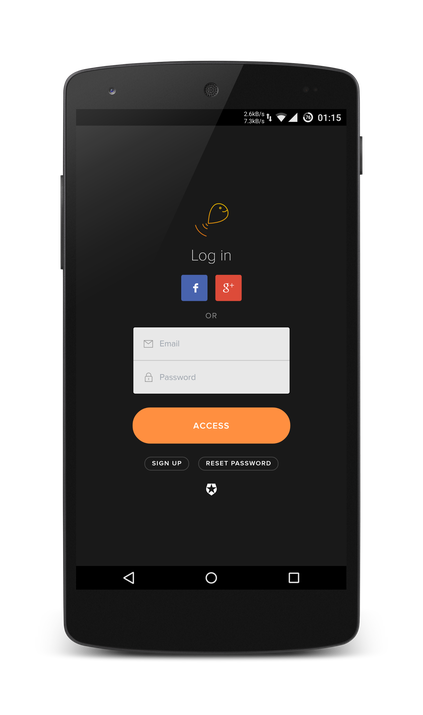
\includegraphics[width=0.45\textwidth]{./img/loginframed.png}
\caption{Login screen}
\label{fig:loginscreen}
\end{figure}

For the login page will be using auth0 authentication.  There is a template provided by auth0 to implement for these purposes. This template can be changed if needed and themed to the developers liking.  We have kept it very simple with small changes to the background and the addition of a logo.

This screen already takes care of the clean look that Choona is aiming for, the form is laid out very well with all the buttons arranged so that the user is not confused. A clear distinction is made between logging on via a social network or through an email address (both need to be available). The sign-in button is clear and well placed and makes use of the Choona orange which ties up our theme.\\

\clearpage

\noindent\underline{Side menu page}\newline

\noindent
\begin{figure}[h!]
\centering
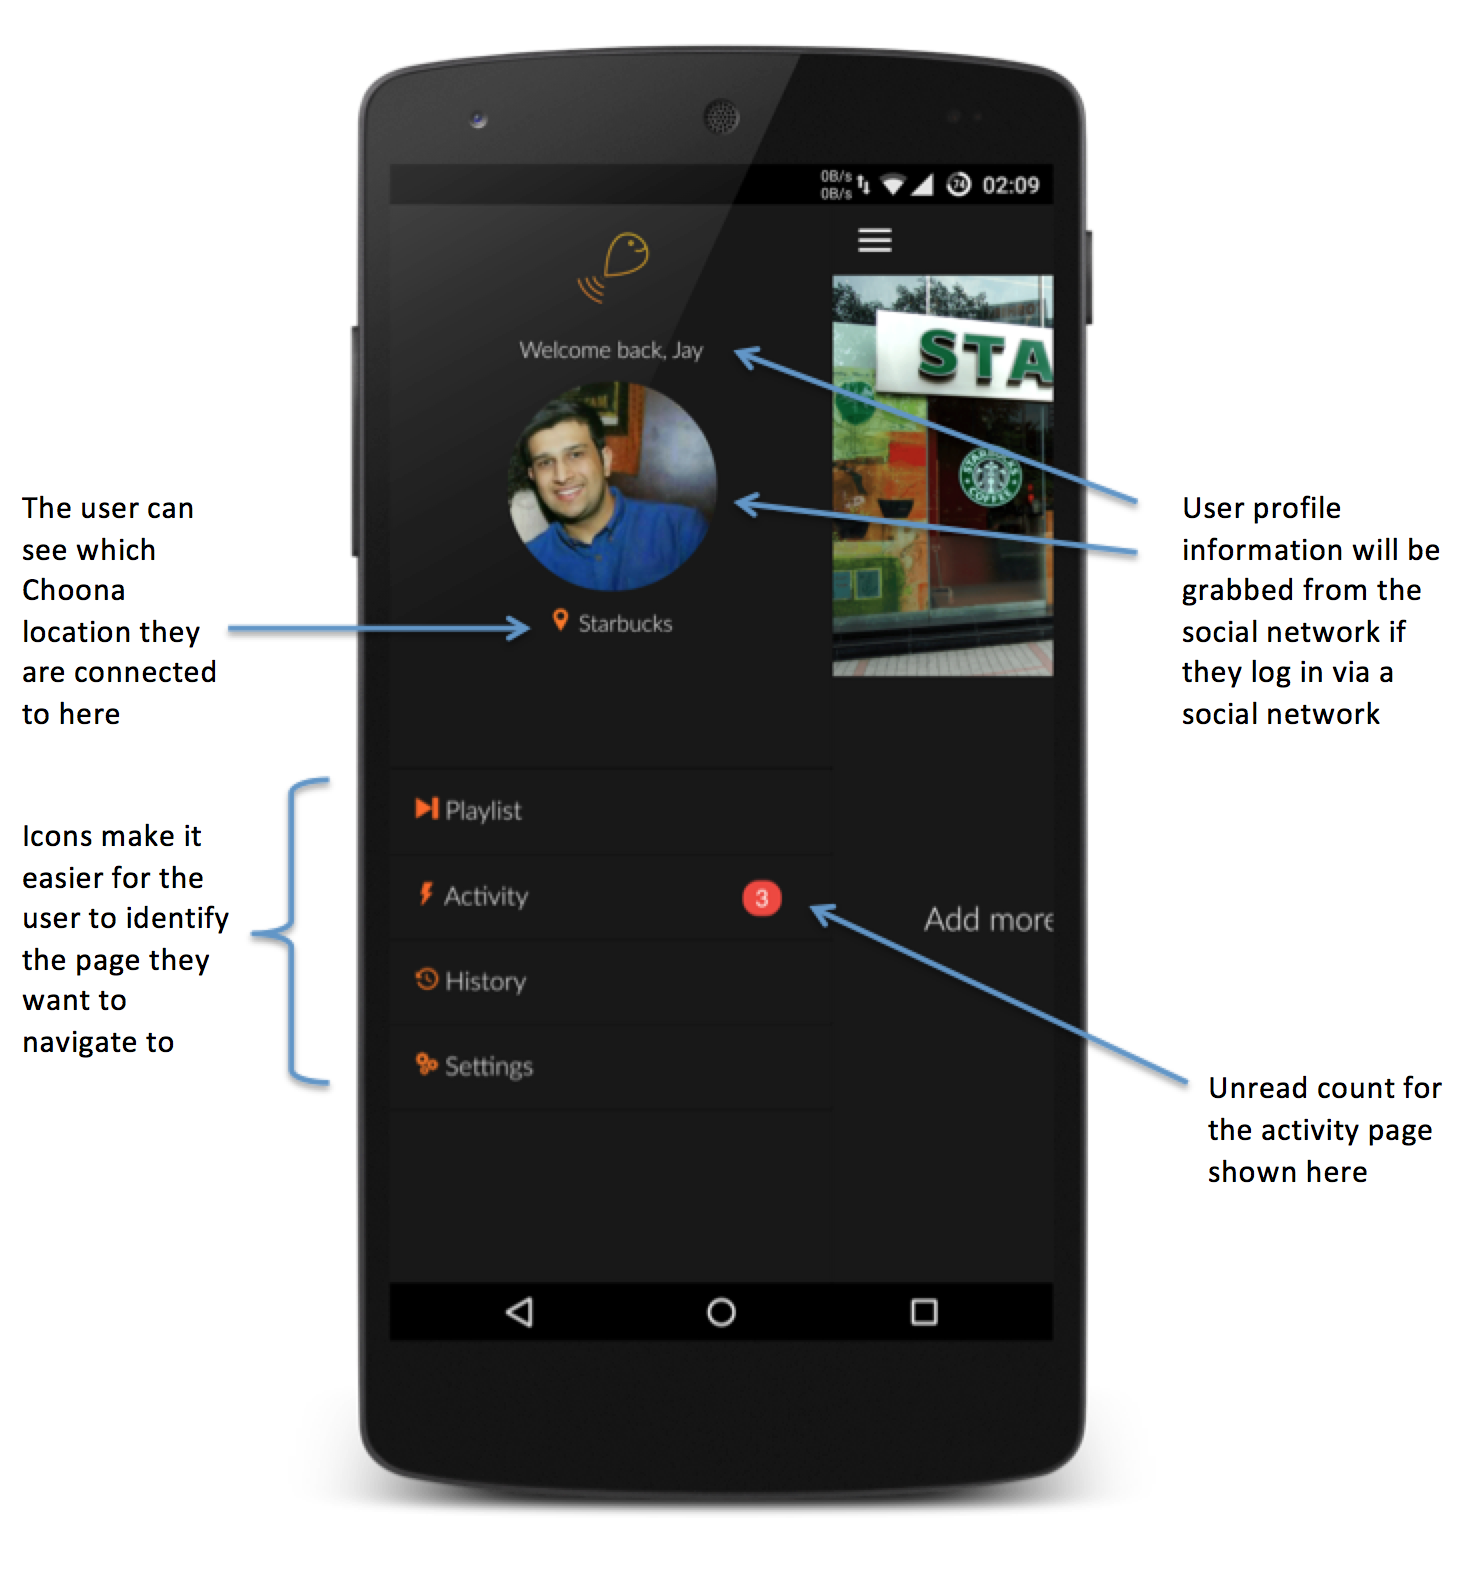
\includegraphics[width=0.76\textwidth]{./img/sidemenuannotated.png}
\caption{Side menu page}
\label{fig:sidemenu}
\end{figure}

The side menu page will be used by the user to navigate the app. It's important that this page is simple and straight forward or the user will not be able to find what they need or do what they want. The profile section positioned at the top assures the user they are logged in and welcomes them to Choona.  Below the profile image, the name of the Choona location they are currently connected to will be shown. Moving down the screen, all the different pages are listed. Each page has an icon, this makes it visually easy for the user to move to different pages and also to identify the pages. Additionally on the activity page, an unread count is shown in the side menu so the user knows if there are any unread activities.\\

\clearpage

\noindent\underline{Playlist page}\newline

\noindent
\begin{figure}[h!]
\centering
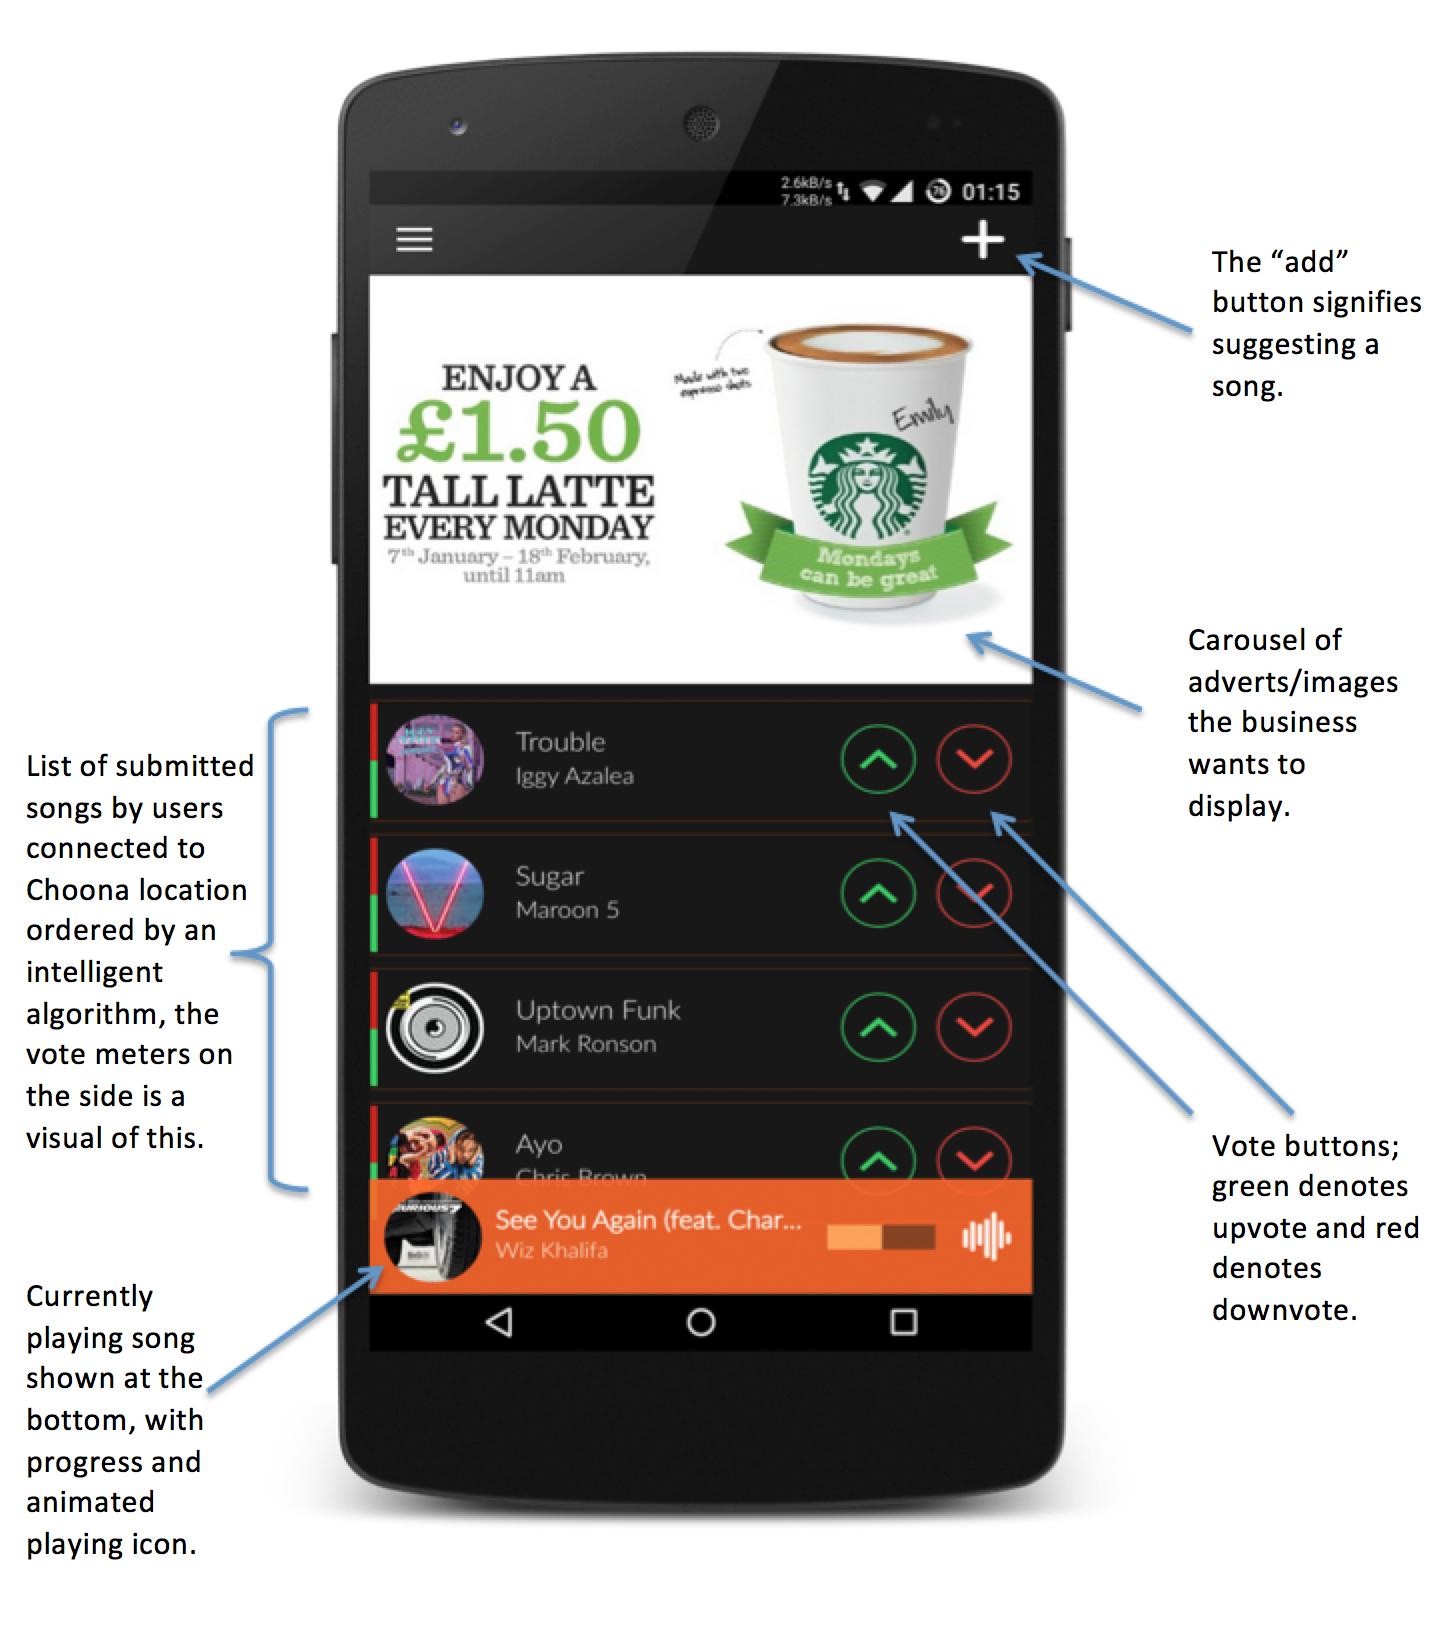
\includegraphics[width=0.65\textwidth]{./img/playlistannotated.png}
\caption{Playlist page}
\label{fig:playlist}
\end{figure}

This is one of the most important pages in the application, here the user will be able to vote on the songs suggested and also have access to the search page where they will be able to add a song. From the top, the user will see a carousel of images which the business will set up beforehand, this could be adverts for the business. Below there will be the list of suggested songs by others. These are in a list with each song containing an up-vote and down-vote button.  Everything is spaced evenly so the user can scroll and vote with ease. The user is also presented with a live vote-meter on the left of every song item in the list. This adds another dimension to the app where they can visually see how well that track is doing (more votes = higher up the list); denoted by appropriate green and red bars in the `votemeter'. Finally at the bottom, the now playing bar shows the current song being played. This bar can be tapped on to access the now playing page; this is conventional in most music applications, such as Google play music.

\clearpage


\noindent\underline{Search page}\newline

\noindent
\begin{figure}[h!]
\centering
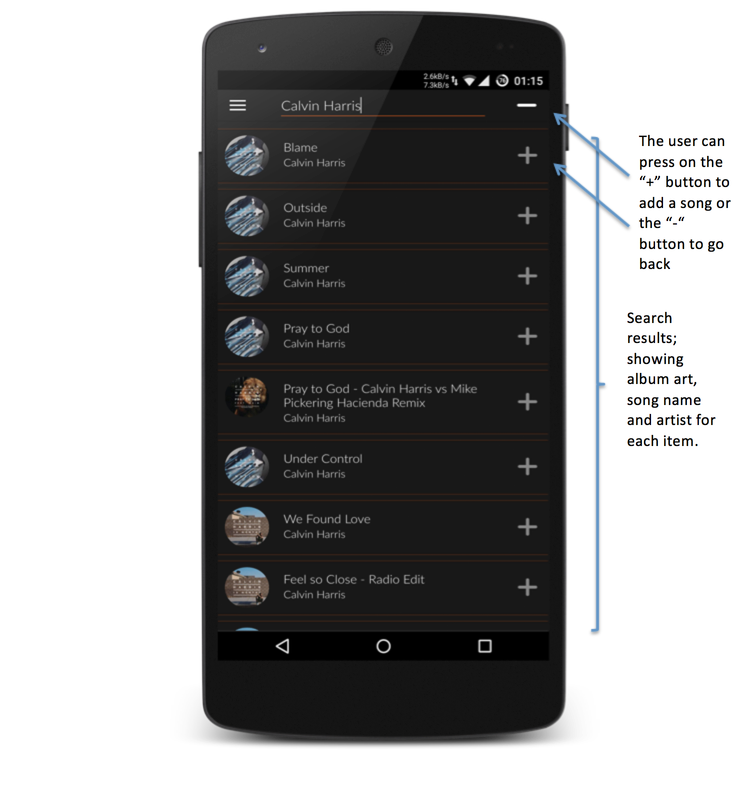
\includegraphics[width=0.7\textwidth]{./img/searchannotated.png}
\caption{Search page}
\label{fig:searchpage}
\end{figure}

Through this page, the user will add a song, thus it is important that this screen is easy to follow. When the user starts typing all the results will be shown as indicated in figure \ref{fig:searchpage}. Beside each song, a `+' sign will appear, similar to the one on the playlist page signifying they want to add that song to the playlist. The `-' button can be used to got back and cancel the search. 

This is a very simple approach to the search page and by only showing the vital information, the user does not get overloaded with information. An alternative solution here would be to display fuller album covers but this would mean more space will be taken per item which would make it harder for users to scroll through all the search results. Thus this solution would be friendlier to smaller screen devices.

\clearpage

\noindent\underline{Now playing page}\newline

\noindent
\begin{figure}[h!]
\centering
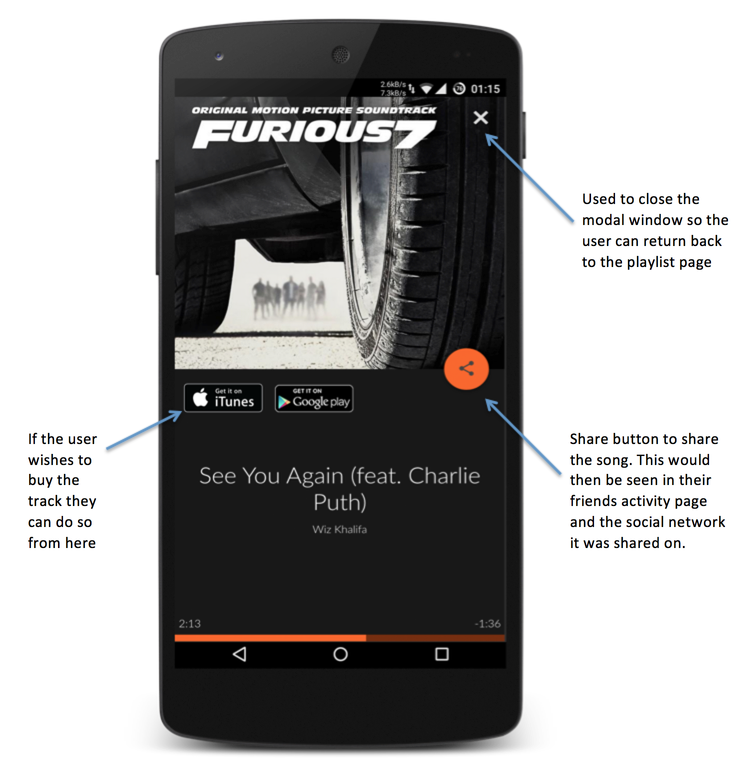
\includegraphics[width=0.8\textwidth]{./img/nowplayingannotated.png}
\caption{Now playing page}
\label{fig:nowplaying}
\end{figure}

The aim of this page is to show clear artwork and song information to the user. Furthermore there will be links to buy the song (one of the revenue streams for Choona) and also to share what they are listening to and where. The share button will be placed as a floating button much like the android lollipop ecosystem. Taking all this mind, a very minimal approach for the screen is taken here, spreading the information across the page and making use of the screen real estate. There is also a track scrubber at the bottom of the page, not responsive to the users touch as the business is in control of the music, it is only there to let the user know how far the song has progressed.   

\clearpage

\noindent\underline{Activity page}\newline

\noindent
\begin{figure}[h!]
\centering
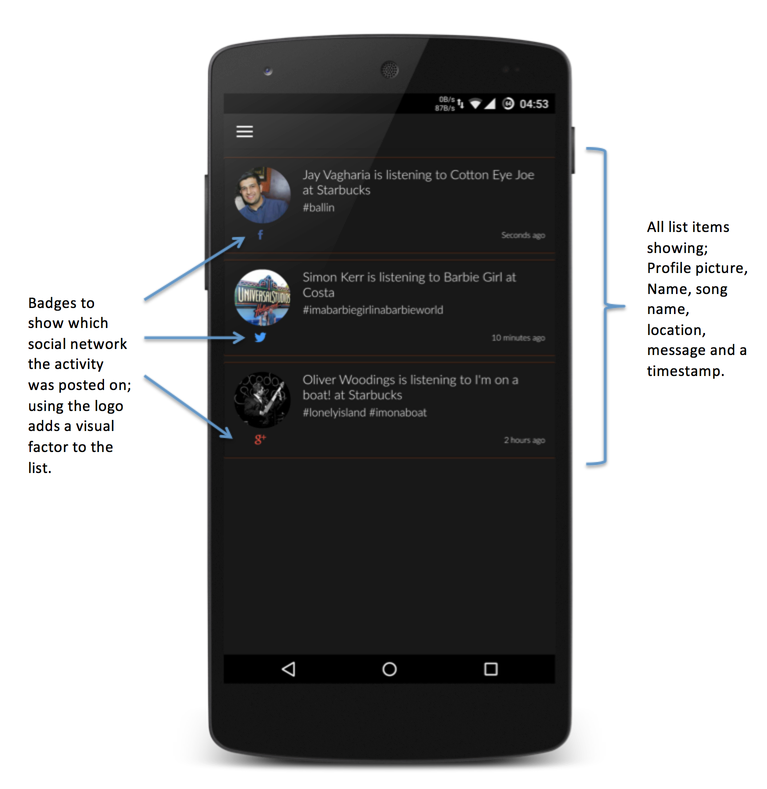
\includegraphics[width=0.8\textwidth]{./img/activityannotated.png}
\caption{Activity page}
\label{fig:activitypage}
\end{figure}

Here is all the Choona activity of the users friends will be shown. This is represented as a clear feed of items containing information to identify their friend the song and their location. An activity item will be placed on this page when the user's friend decides to use the share button on the now playing page which will fire the event. The activity will also be shared on the social network the user sent it to; letting the businesses promote themselves. 

The page follows the global colour scheme and also lays out all the information similar to the list of songs on the playlist page, the use of social badges makes it easy for the user to identify the social network their friends activity was shared on. 
\clearpage

\noindent\underline{History page}\newline

\noindent
\begin{figure}[h!]
\centering
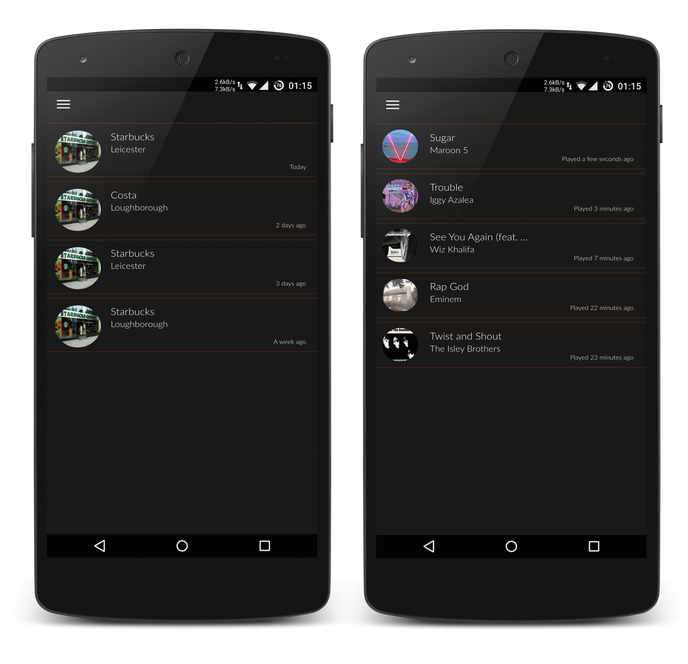
\includegraphics[width=0.77\textwidth]{./img/historyboth.png}
\caption{History pages}
\label{fig:historyboth}
\end{figure}

This page lets the user easily access any songs that were played in places they visited in the last week. First they will be shown a list of places (Left on figure \ref{fig:historyboth}) and then they can tap on a certain place to see the songs played in the time they were there (right on figure \ref{fig:historyboth}. Simple lists were used here taking the minimal approach with only showing data that the user is interested in. The styling is consistent with the other pages that employ lists in their containers.

An alternative design here would be an accordion approach where each root item would be a location and when expanded, would show all the songs played for that location for the duration that the user was there. Even though this method means that the user does not have to visit another page, it could be be very bad for scrolling through a long list of items. This would be unpopular with smaller screen phones as they will have to scroll through a lot more to find what they want.

\clearpage

\noindent\underline{Settings page}\newline

\noindent
\begin{figure}[h!]
\centering
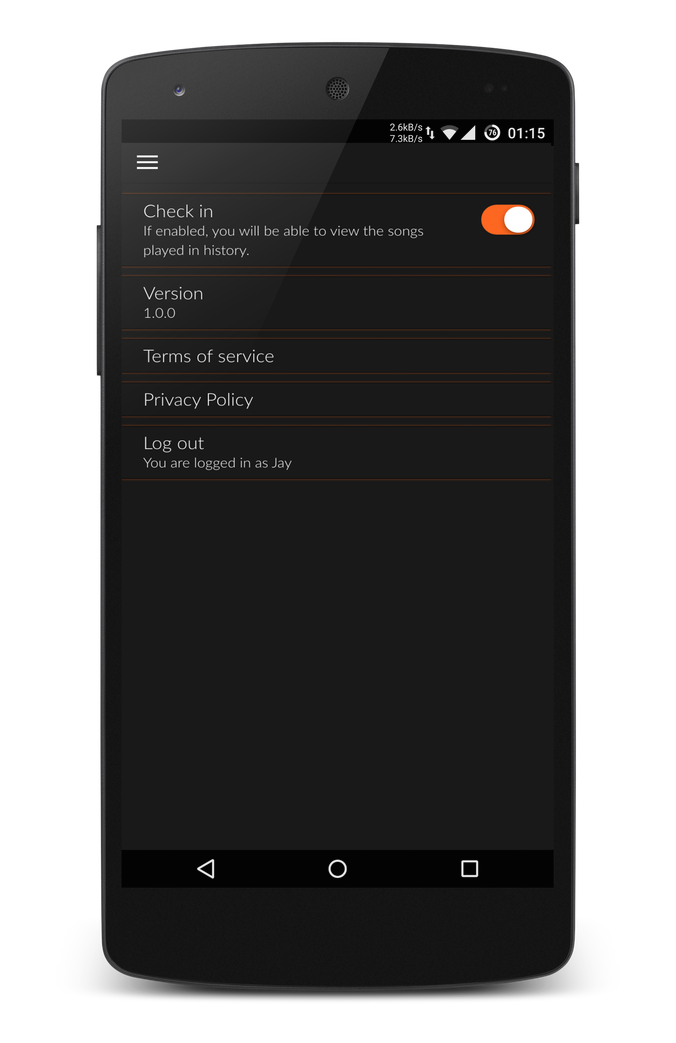
\includegraphics[width=0.55\textwidth]{./img/settingsframed.png}
\caption{Settings page}
\label{fig:settingspage}
\end{figure}

This is where the user will be able to configure the app and any options around it. At this point there are minimal things to configure on the app. One option is to toggle auto logging of history which is on by default but the user can turn it off if they wish. This is a slider button familiar to both android and iOS devices for toggling something. The log out button will also belong here in the case they want to log in with another account. 

This is another simple screen on the phone, so a minimal approach has been taken to design it. Other than the options talked about above, important information such as Choona's terms of service and privacy policy are also included in this screen.